\documentclass[t]{beamer}
\usetheme{Copenhagen}
\setbeamertemplate{headline}{} % remove toc from headers
\beamertemplatenavigationsymbolsempty

\usepackage{amsmath, array, tikz, bm, pgfplots, tcolorbox, graphicx, venndiagram, color, colortbl, xfrac}
\pgfplotsset{compat = 1.16}
\usepgfplotslibrary{statistics}
\usetikzlibrary{calc}

\title{Other Probability Distributions}
\author{}
\date{}

\AtBeginSection[]
{
  \begin{frame}
    \frametitle{Objectives}
    \tableofcontents[currentsection]
  \end{frame}
}

\begin{document}

\begin{frame} 
\maketitle
\end{frame}

\section{Solve problems involving geometric probability distributions}

\begin{frame}{Binomial vs. Geometric Distributions}
With binomial distributions, we had the following conditions:
	\begin{itemize}
		\item There are a fixed number of $n$ repeated independent trials
		\item Each trial's outcome is either a success or failure
		\item The probability of success, $p$, never changes
	\end{itemize}	
	\vspace{10pt}
\onslide<2->{We could calculate the probability of obtaining 8 heads out of 10 flips of a coin.}	\newline\\
\onslide<3->{One of these outcomes is TTHTHHHTTH.}	
\end{frame}

\begin{frame}{Binomial vs. Geometric Distributions}
With geometric distributions, we would interested in the probability of obtaining our first success (flipping a tail) after $x$ flips of the coin.	\newline\\	
\onslide<2->{To put it another way, a geometric distribution has the following property:}
\onslide<3->{\[\underbrace{FFF \cdots F}_{x-1 \text{ failures}}S\]}
\end{frame}

\begin{frame}{Geometric Distributions}
The probability of obtaining our first success after $x$ binomial experiments is given by
\[P(X=x) = (1-p)^{x-1} \cdot p\]
\end{frame}

\begin{frame}{Example 1}
A student is given a 10-question multiple choice test in which each question has 5 possible answers. What is the probability that the first question the student guesses correctly on the 4th question?	\newline\\

FFFS	

\begin{align*}
P(X = 4) &= (1-0.2)^4 (0.2)	\\
&= 0.08192
\end{align*}
\end{frame}

\begin{frame}{Bar Graph of Example 1}
\begin{center}
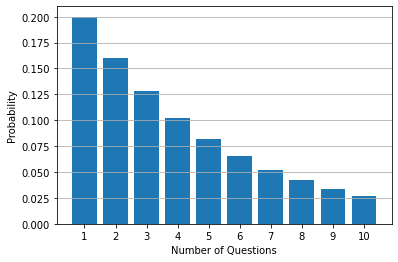
\includegraphics[scale=0.6]{../Images/geometric_mult_choice.png}
\end{center}
\end{frame}

\begin{frame}{Mean and Standard Deviation of Geometric Distributions}

\end{frame}

% Geometric Distributions
% Hypergeometric Distributions
% Poisson Distributions

\end{document}